% Modelo de relatório no estilo artigo em duas colunas
\documentclass[twocolumn]{article}
%\usepackage[portuguese]{babel}
\usepackage[utf8]{inputenc}
\usepackage{amsmath}
\usepackage{minted}
\usepackage{algorithm}
\usepackage{algorithmic}
\usepackage{subcaption}
\usepackage{mathtools}
\usepackage{graphicx}
\usepackage{color}
\usepackage{authblk}
\usepackage[colorlinks,citecolor=red,urlcolor=blue,bookmarks=false,hypertexnames=true]{hyperref}
\usepackage{geometry}
% Tamanho das margens:
\geometry{
	a4paper,
	total={185mm,260mm},
	left=15mm,
	top=15mm,
}
%%%%%%%%%%%%%%%%%%%%%%%%%%%%%%%%%%%%%%%%%
% Bibliografia estilo ABNT. Se não tiver instalado, comente a linha abaixo.
\usepackage[alf, abnt-etal-list=0, abnt-emphasize=bf,abnt-last-names=bibtex, abnt-etal-text=it, abnt-etal-cite=2]{abntex2cite}
%%%%%%%%%%%%%%%%%%%%%%%%%%%%%%%%%%%%%%%%%

% Dados de identificação
\title{3F8 Inference: Coursework}
\author{Vatsal Raina}

\begin{document}

\maketitle        

\section{Introduction}

The coursework exercise investigates a typical binary classification problem where a data set of 1000 points is provided. The data points are randomly split into 800 points for the training data set and 200 points for the test data set. The classification is at first attempted using a linear Logistic Classification model. Significant improvement is made when the logistic classification model is used with the inputs expanded through a set of radial basis functions (RBFs) centred on the training data points.

\section{Part \textit{a}}

The logistic classification model is used, which uses the sigmodial logistic function to define the probabilities of $y^{(n)}\in\{1,0\}$.
$$ P(y^{(n)}=1|\Tilde{x}^{(n)})=\frac{1}{1+e^{-\beta^T\Tilde{x}^{(n)}}}=\sigma(\beta^T\Tilde{x}^{(n)}) $$
$$ P(y^{(n)}=0|\Tilde{x}^{(n)})= 1- \sigma(\beta^T\Tilde{x}^{(n)})=\sigma(-\beta^T\Tilde{x}^{(n)})$$
Using the above definitions, an expression of the likelihood of all the data can be determined as the product of the likelihood of each individual data point.
$$P(y|X,\beta)=\prod_{n=1}^N P(y^{(n)}|\Tilde{x}^{(n)}) $$
$$P(y|X,\beta) = \prod_{n=1}^N \sigma(\beta^T\Tilde{x}^{(n)})^{y^{(n)}}(1-\sigma(\beta^T\Tilde{x}^{(n)}))^{1-y^{(n)}}$$

The aim is to find the parameters $\beta$ that maximise the above expression. This is equivalent to maximising the log of the likelihood as the log function is monotonically increasing. Hence, it is desired to compute $\frac{\partial}{\partial \beta}\mathcal{L}(\beta)$ where $\mathcal{L}(\beta)=\text{log}P(y|X,\beta)$. The derivative can then be set to zero and solved numerically using methods such as gradient ascent.
$$\mathcal{L}(\beta)=\sum_{n=1}^N y^{(n)}\text{log}\left[\sigma(\beta^T\Tilde{x}^{(n)})\right]+(1-y^{(n)})\text{log}\left[1-\sigma(\beta^T\Tilde{x}^{(n)})\right]$$
$$\mathcal{L}(\beta)=\sum_{n=1}^N y^{(n)}\text{log}\left[\sigma(\beta^T\Tilde{x}^{(n)})\right]+(1-y^{(n)})\text{log}\left[\sigma(-\beta^T\Tilde{x}^{(n)})\right]$$
Using $\frac{d\sigma (x)}{dx}=\sigma(x)(1-\sigma(x))$ gives,
$$\frac{\partial}{\partial \beta}y^{(n)}\text{log}\left[\sigma(\beta^T\Tilde{x}^{(n)})\right]=y^{(n)}(1-\sigma(\beta^T\Tilde{x}^{(n)}))\Tilde{x}^{(n)}$$
$$\frac{\partial}{\partial \beta}\mathcal{L}(\beta)=\sum_{n=1}^N\left[(y^{(n)}-\sigma(\beta^T\Tilde{x}^{(n)})\right]\Tilde{x}^{(n)}$$

\section{Part \textit{b}}

\subsection{Pseudo-code}

The following pseudo-code outlines the procedure to estimate the parameters $\beta$ using gradient ascent of the log-likelihood $\beta^{\text{new}}=\beta^{\text{old}}+\eta\frac{\partial}{\partial \beta}\mathcal{L}(\beta^{\text{old}})$. In order to use vectorised code, it is convenient to express the gradients of the log-likelihood of the parameters in vector form.
$$\frac{\partial}{\partial \beta}\mathcal{L}(\beta)=\Tilde{X}^T(y-\sigma(a))$$
where $\Tilde{X}$ is a matrix of the input variables prepended with a column of 1s, $y$ is a vector of the corresponding outputs and $\sigma(a)$ is a vector of the logistic function applied to the activations $a=\Tilde{X}\beta$. Algorithm 1 assumes the logistic function has been defined. The data is held in matrix $X$ and the outputs are held in the vector $y$.

\begin{algorithm}
\caption{Vectorised Gradient Ascent}
\begin{algorithmic}
\STATE $N\leftarrow X$.rows
\STATE ones $\leftarrow \left[1\right]*N$
\STATE $\Tilde{X}\leftarrow$ append(ones, $X$, axis=1)
\STATE $\beta\leftarrow \left[0\right]*\Tilde{X}$.columns
\STATE $\eta\leftarrow1/N$
\STATE steps $\leftarrow 1000$
\FOR{$i=$ 1 to steps}
\STATE $a \leftarrow \Tilde{X}\beta$
\STATE sigs $\leftarrow$ $\sigma(a)$
\STATE $dL/d\beta \leftarrow \Tilde{X}^T(y-\text{sigs})$
\STATE $\beta\leftarrow\beta+\eta*dL/d\beta$
\ENDFOR
\RETURN $\beta$
\end{algorithmic}
\end{algorithm}

\subsection{Learning rate}
A good learning rate, $\eta$, is vital in the gradient ascent algorithm. If the learning rate is too small, the algorithm may take a very long time to converge to the maximum of the log likelihood, resulting in a waste of resources. If the learning rate is too large, the algorithm may never converge as consecutive steps may miss the maximum and cause the algorithm to oscillate indefinitely. In general, there is no rule which can be used to deduce the optimal learning rate.

A possible approach to find an appropriate learning rate may involve training the model initially with a very low learning rate and increasing it (either linearly or exponentially) in consecutive iterations. A justification for this approach is that $\frac{\partial \mathcal{L}}{\partial \beta}$ becomes very small near the maximum, which slows down the rate of convergence.

Another method is to change the learning rate every iteration according to a given cyclic function. Each cycle of the function lasts a discrete number of iterations. Consequently, the learning rate varies between an upperbound and a lowerbound. This enables traversing saddle points effectively.

If a constant learning rate is desired, a simple approach is to set $\eta\propto \frac{1}{N}$. The drawback of this approach is that the learning rate can be very slow for large data sets.

The general aim is to reach find the weights which minimise the likelihood of the data in fewest iterations as possible. The gradient ascent algorithm can be modified to the stochastic gradient ascent algorithm. The difference is that the stochastic algorithm computes the log likelihood using a random subset of the data points at each iteration, which permits a significant reduction in the order of complexity.

\section{Part \textit{c}}

\begin{figure}[!htb]
	\centering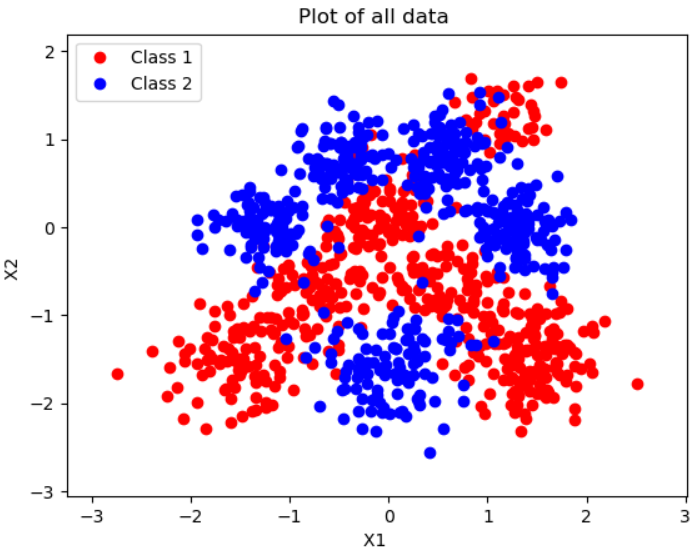
\includegraphics[width=\columnwidth]{1}\\
	\caption{Scatter plot of data classifed as one of two classes}\label{triangulo}
\end{figure}

Figure 1 depicts the 1000 data points available in the data set which belong to one of two classes. This graphical representation is only possible because each data point has only two input variables. The aim is to develop a classifier which will be able to accurately predict the class of a new data point.

A classifier with a linear class boundary is likely to perform very poorly on the data in figure 1 because the data belonging to each class is clearly not separated by a straight line. The data in class 2 appears to surround the data in class 1. However, there are clearly regions where data is more likely to belong to one class, which indicates a non-linear classifier would be significantly more appropriate for this classification problem.

\section{Part \textit{d}}

In order to train the linear classifier using the logistic classification method, it is required the data is split into training and test sets. An appropriate ratio is 4:1, which gives 800 training points to determine the optimal value of the weights and 200 test points which can be used to measure the success of the trained weights. The below Python code randomly generates the training and test data sets by first zipping the outputs vector to the inputs matrix and then shuffling the combined structure prior to partitioning the matrix to extract the shuffled inputs and outputs. 

\begin{minted}{python}
    X,y = load_data()
    # Split data into training and test randomly
    # Create supermatrix of inputs and outputs
    y = y.reshape(X.shape[0],1) 
    yX = np.append(y,X,axis=1)
    # Randomly shuffle the values
    shuffle(yX)
    # Extract the outputs and inputs
    y = yX[:,0]
    X = yX[:,1:]
    X_train = X[:800]
    y_train = y[:800]
    X_test = X[800:]
    y_test = y[800:]
\end{minted}

The following code implements the gradient ascent pseudo-code from section 3.1 into Python. Some modifications exist in the code in order to store a history of all the weights values, test likelihoods and training likelihoods.

\begin{minted}[breaklines]{python}
def grad_asc(X_train,y_train,X_test,y_test):
    N = X_train.shape[0]
    ones_train = np.ones(shape = (N,1))
    # Concatenate ones vector to data matrix
    X_train=np.append(ones_train,X_train,axis=1)   
    ones_test=np.ones(shape=(X_test.shape[0],1))
    X_test = np.append(ones_test,X_test,axis=1)
    # Initialise weights to zero
    w = np.array([0.0]*X_train.shape[1])  
    eta = 1/N   # Set learning rate
    iterations = 100 
    w_hist = []  # List for weights at each step
    log_liks_train = []
    log_liks_test = []
    for i in range(iterations):
        log_liks_train.append( compute_average_ll(X_train,y_train,w))
        log_liks_test.append( compute_average_ll(X_test,y_test,w))
        w_hist.append(w)
        # Find logistic function of each activation
        logists = logistic(X_train.dot(w))
        # Get derivative
        dl_dw = (X_train.T).dot(y_train-logists)
        w += eta * dl_dw    # Update step
    return np.array(w_hist), np.array(log_liks_train), np.array(log_liks_test)
\end{minted}

Using the lists \texttt{log\_liks\_train}[] and \texttt{log\_liks\_test}[], it is straightforward to report the training curves showing the log-likelihood on training and test datasets per datapoint as the optimisation proceeds. It is important to note that the log-likelihood at each iteration has been averaged over the number of data points in order to be able to have a meaningful value to compare against other classifiers which may use a different number of data points for the training and test data sets.

\begin{figure}[!htb]
	\centering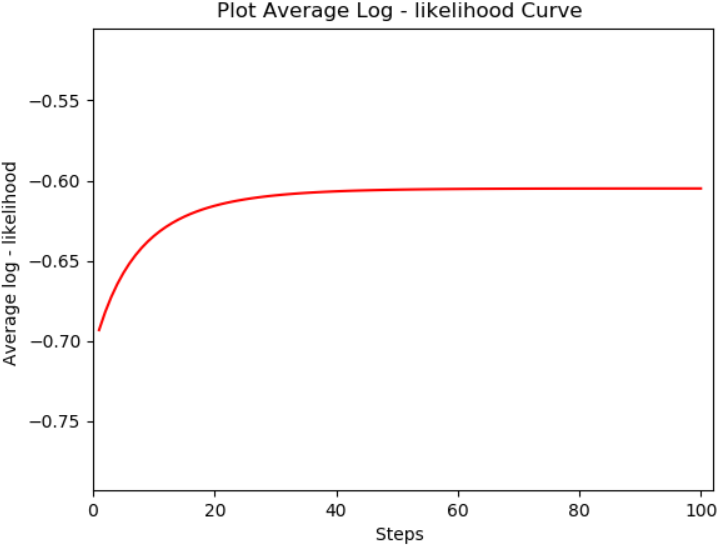
\includegraphics[width=\columnwidth]{b}\\
	\caption{Linear classifier - Training data log-likelihood}\label{triangul}
\end{figure}

\begin{figure}[!htb]
	\centering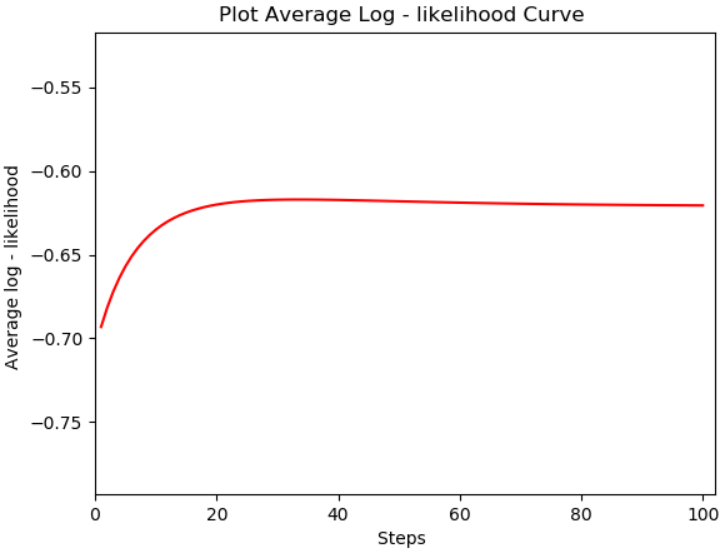
\includegraphics[width=\columnwidth]{c}\\
	\caption{Linear classifier - Test data log-likelihood}\label{triangu}
\end{figure}

From figure 2, it is clear that the mean training log-likelihood increases with each iteration until it plateaus to a maximum value. The plateau is expected as it suggests that the weights vector has converged to a value which maximises the likelihood of the training data. However, the largest log likelihood reached by the training data is -0.611 while a value of 0 is the ideal value. This large deviation from the desired value suggests that the linear model is inappropriate as the weights vector is unable to sufficiently maximise the likelihood of the data points. The test data log likelihoods are displayed in figure 3. A similar behaviour is depicted to figure 2 where the training data log likelihood plateaus once the weights vector has reached a constant value. The final value of the test log likelihood is lower than the corresponding value of the training log likelihood as the model will perform better on the training data than the test data given that the weights were tuned using the training data.

\begin{figure}[!htb]
	\centering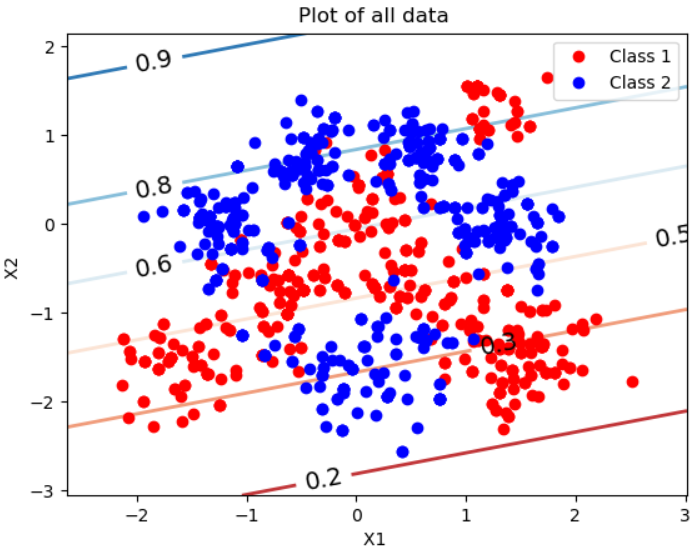
\includegraphics[width=\columnwidth]{d}\\
	\caption{Linear classifier probability contours on all data}\label{triang}
\end{figure}

The labelled straight lines in figure 4 depict the results of the linear classifier after being trained on the training data. Recall, the second and third components of the weights vector form a vector which should be orthogonal to the decision boundary lines. The label on each of the lines in figure 4 informs the probability the classifier assigns a data point at the respective position belonging to class 2 (in blue). Hence, the straight line labelled 0.5 corresponds to the decision boundary, which suggests that everything below the line should belong to class 1 and everything above the line should belong to class 2.

Visually inspecting the decision boundary lines in figure 4, it is clear that the linear classifier has performed very poorly on the data. For example, the straight line labelled 0.8 passes through a cluster of points belonging to class 1. This means that the classifier assigns a probability of 0.8 belonging to class 2 for a new data point in this small cluster of class 1 points. It is not surprising that the linear classifier appears to have performed very poorly on the data because there is no clear straight line which can appropriately divide the data belonging to each class. 

\section{Part \textit{e}}

The final training are test log-likelihoods per datapoint are as follows:
$$\textbf{Training:}-0.611\hspace{15pt} \textbf{Test:}-0.658$$

For the test data, a threshold is applied to the probabilistic predictions such that a test data point with a corresponding output greater than $\frac{1}{2}$ is assigned $\hat{y}=1$ and is otherwise assigned $\hat{y}=0$. This allows the confusion matrix to be defined as below.

$$\begin{bmatrix} P(\hat{y}=0|y=0) & P(\hat{y}=1|y=0) \\ P(\hat{y}=0|y=1) & P(\hat{y}=1|y=1) \end{bmatrix}$$

The trace (sum of diagonal elements) of the confusion matrix gives a measure of how well the classifier performs on the test data. The sum of the off-diagonal terms in the confusion matrix gives a measure of how poorly the classifier performs. The confusion matrix for the linear classifier is given below.
$$\texttt{conf}_{\text{linear}}=\begin{bmatrix} 0.576 & 0.424 \\ 0.296 & 0.704 \end{bmatrix}$$
Hence, the fraction of incorrectly classified test data points is $0.424$ when $y=0$ and $0.296$ when $y=1$, which is quite high given a random classifier can expect to have an error rate of 0.5. The Python code to produce the confusion matrix is given below.

\begin{minted}[breaklines]{python}
def get_y_hat(X_test,w):
    ones = np.ones(shape = (X_test.shape[0],1))
    X_test = np.append(ones,X_test,axis=1)
    y_hat = logistic(X_test.dot(w))
    for i,y in enumerate(y_hat):
        if y<0.5: y_hat[i] = 0
        else: y_hat[i] = 1
    return np.array(y_hat)

def confusion_matrix(y_test,y_hat):
    con_mat = np.array([[0.0,0.0],[0.0,0.0]])
    N = y_test.shape[0]
    N_1 = np.sum(y_test)
    N_0 = N - N_1
    for i in range(N):
        diff = abs(y_test[i]-y_hat[i])
        if y_test[i] == 0:
            if diff ==0: con_mat[0][0]+=1
            else: con_mat[0][1]+=1
        else:
            if diff ==0: con_mat[1][1]+=1
            else:con_mat[1][0]+=1
    con_mat[0] = con_mat[0]/N_0
    con_mat[1] = con_mat[1]/N_1
    print(con_mat)

\end{minted}

\section{Part \textit{f}}

The results so far have indicated in several forms that a linear classifier is inappropriate for the data. A more suitable model is to use a non-linear classification method. One possible method is to expand the inputs through a set of radial basis functions (RBFs) centred on the training datapoints. Hence, the matrix $\Tilde{X}$ now has $N_{train}+1=801$ columns. The additional column is for the column of ones to account for the bias weight term. Thus, the first column of $\Tilde{X}$ is a column of 1s while the remaining entries can be described by the following form.
$$\tilde{x}^{(n)}_{m+1}=\text{exp}\left(-\frac{1}{2l^2}\sum_{d=1}^{2}(x_d^{(n)}-x_d^{m})^2\right)$$
Note, the paramter $l$ is of importance because it can be interpreted as the variance of the radial basis function centred on a given training datapoint. The Logistic Classification model has weights trained using the feature-expanded inputs for $l\in\{0.01,0.1,1\}$. It is necessary to decrease the learning rate for larger values of $l$ in order to avoid overstepping the maximum point in the log-likelihood of the training data.

\begin{figure}[!htb]
	\centering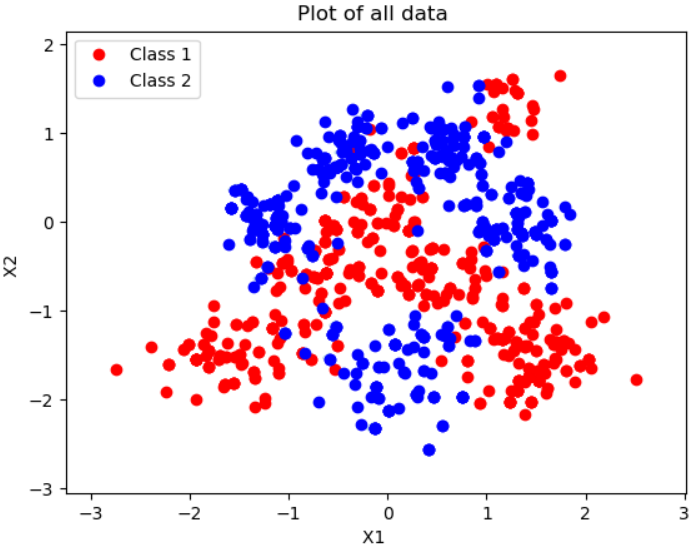
\includegraphics[width=\columnwidth]{2}\\
	\caption{Non-linear classifier with $l=0.01$}\label{trian}
\end{figure}

\begin{figure}[!htb]
	\centering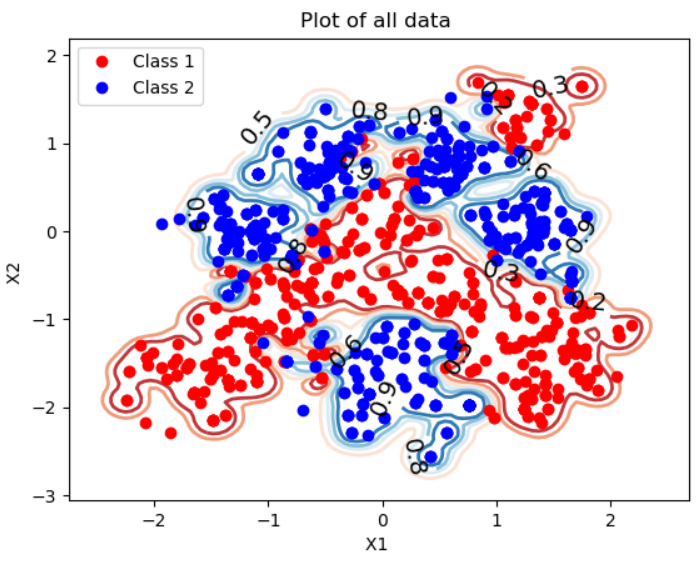
\includegraphics[width=\columnwidth]{3}\\
	\caption{Non-linear classifier with $l=0.1$}\label{tria}
\end{figure}

\begin{figure}[!htb]
	\centering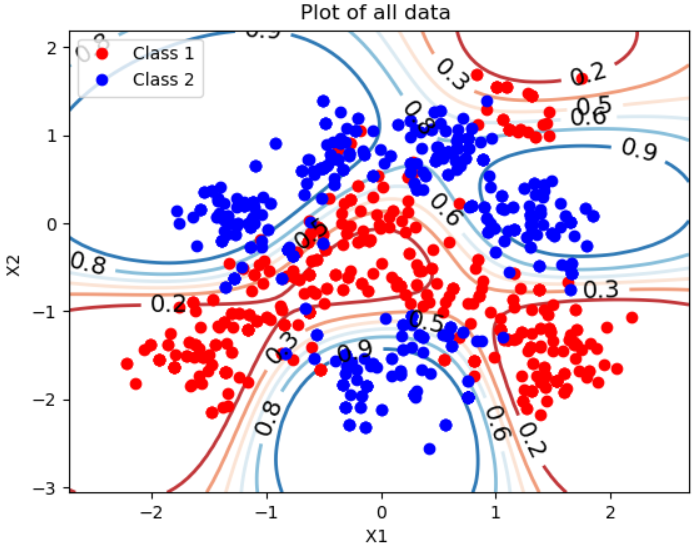
\includegraphics[width=\columnwidth]{4}\\
	\caption{Non-linear classifier with $l=1$}\label{tri}
\end{figure}

The probabilistic decision boundary lines are not visible in figure 5 for $l=0.01$ because the decision boundary lines are faint and only around individual training data points. This makes sense intuitively as the variance of the radial functions is set to be very small with $l=0.01$. From visually comparing figures 5,6 and 7, it is clear that the decision boundary lines appear to perform best when $l=1$. Best results occur for $l=1$ because it allows sufficient variance for the radial functions centred around the training data points.

\section{Part \textit{g}}

In order to quantitatively compare the performance of the non-linear classifier for different values of $l$, table 1 depicts the training likelihood, test likelihood and the confusion matrix for each value of $l$.

\setlength{\tabcolsep}{2pt}
\setlength{\arrayrulewidth}{0.5mm}
\renewcommand{\arraystretch}{1.5}
\begin{table}[h!]
    \centering
    \begin{tabular}{|c|c|c|c|}
    \hline
    $l$ & Training likelihood & Test likelihood & Confusion matrix \\
    \hline\hline
       0.01  &  -0.189 & -0.507 & $\begin{bmatrix} 0.484 & 0.516 \\ 0.00952 & 0.990 \end{bmatrix}$\\ \hline
      0.1  &  -0.102 & -0.310 & $\begin{bmatrix} 0.924 & 0.0761 \\ 0.111 & 0.889 \end{bmatrix}$\\ \hline
       1  &  -0.0369 & -0.209 & $\begin{bmatrix} 0.917 & 0.0833 \\ 0.0577 & 0.942 \end{bmatrix}$\\ \hline   
    \end{tabular}
    \caption{Performance of classifier for $l\in\{0.01,0.1,1\}$}
    \label{tab:my_label}
\end{table}

Using table 1, it is clear that as the value of $l$ increases, the training and test likelihoods get closer to the desired value of 0. Similarly, the trace of the confusion matrix increases with increasing $l$ to the ideal value of 2. For example, the non-linear classifier with $l=1$ correctly classifies 91.7\% of test data point when $y=0$ and 94.2\% when $y=1$. This is equivalent to a trace of $0.917+0.942=1.86$ (maximum value possible is 2). This confirms the visual observations from figures 5,6 and 7 where the decision boundary lines best classified the data points for $l=1$.

In comparison to the confusion matrix for the original inputs for the linear classifier, the trace of the confusion matrix was $0.576+0.704=1.28$. As $1.86>>1.28$, it is natural to conclude the non-linear classifier with $l=1$ performs significantly better than the original linear classifier. A similar argument can be made using the log likelihoods as the training log likelihood and the test log likelihood are significantly closer to 0 for the non-linear classifier with $l=1$ compared to the linear classifier.

An interesting discussion is regarding why the non-linear classifier performs so poorly overall with $l=0.01$. It appears the classifier correctly classifies 99\% of test data points when $y=1$ but at the cost of only correctly classifying 48.4\% when $y=0$. The key idea is that the variance of the radial basis functions is so small that they are too focused on the training data points and consequently work very well on one class of data points and extremely poorly on the other class of data points. In other words, a small $l$ results in over-fitting on the training data. An alternative to increasing the value of $l$ is to use Bayesian non-linear classification as a zero mean prior on the weights can help to avoid the weights getting too large in magnitude, which is a typical occurrence in models which have overfit to the training data.

An issue which can arise when using the non-linear classifier with $l=1$ is that the activations may get very large in magnitude, which can lead to taking logs of values very close to zero, which in turn can create numerical errors. The following snippet of Python code indicates how this error is avoided by using the approximation $\text{log}(\sigma(\beta^T\tilde{x}^{(n)}))\rightarrow \beta^T\tilde{x}^{(n)}$ as $\beta^T\tilde{x}^{(n)}\rightarrow\-\infty$.

\begin{minted}[breaklines]{python}
def compute_average_ll (X, y, w):
    output_prob = logistic (np.dot(X, w))
    # Avoid divide by zero
    log_prob=output_prob*1
    log_prob_minus=output_prob*1
    for i,p in enumerate(output_prob):
        if (p<0.0001):
            log_prob[i]=X[i].T.dot(w)
        else:
            log_prob[i] = np.log(output_prob[i])
        if ((1-p)<0.0001):
            log_prob_minus[i]=-X[i].T.dot(w)
        else:
            log_prob_minus[i] = np.log(1.0 - output_prob[i])
    return np. mean (y * log_prob + (1 - y) * log_prob_minus)
\end{minted}

\section{Conclusions}
The following conclusions can be drawn from completing this coursework exercise:
\begin{itemize}
	\item Logistic Classification involves deducing the weights vector which maximises the likelihood of the training data.
	\item Maxmisation of the log-likelihood requires finding the weights vector which sets the gradient to zero. This can be achieved numerically by following methods such as gradient ascent.
	\item Care must be taken to choose the optimal learning rate for gradient ascent such that the maximum value is not overstepped and the algorithm does not run too slowly.
	\item Linear classification performed very poorly on the data because there is no straight line which can divide the two classes of data points.
	\item The non-linear classifier using radial basis functions with $l=1$ offered significant improvements to the linear classifier.
\end{itemize}

\end{document}